%\section{Narrow-band Multi-Target Localization With Distributed Sensors}
\section{Sensor Subset Selection}
\label{sec:SensorSelection}
% \yoav{How is this problem different from the problem of finding the
%   best placement for the sensors in order to maximize the accuracy of
%   localization, ignoring communication bandwidth? }
%   \piya{Majority of existing sensor selection problems (based on submodular optimization, or solving subset selection problem subject to maximum tolerable error bounds) utilize a linear model, where the measurements are {\em linear functions} of the quantity of interest. Target localization is inherently non-linear since the information is contained in phase. Moreover, these algorithms do not give theoretical guarantee on the minimum number of required sensors.}

% With the aim of obtaining a compressive sketch of the correlation matrix (also termed as compressive covariance sensing), we will optimize the design of sensor array (i.e. choice of $\mathbf{d}_m, 1\leq m\leq M$) by understanding how the array geometry controls the algebraic structure of $R_T$. One of the main objectives will be to understand how much communication is needed (and between which subset of sensors) to achieve a certain level of accuracy. To illustrate this, we briefly discuss Co-PI Pal's recent work in structured sampler design (e.g., nested, coprime and generalized nested samplers) which utilize the idea of difference sets.

\yoav{Pia, the description of the difference sets and GNS should be flushed out. By which I mean that the concepts should be described clearly and in sufficient detail that the main results can be stated. On the other hand, details such as 8,9,11 are  distracting.}
%\subsection{Background and Prior Work: Difference Set-Inspired Designs:} 
%I will review some results in the context of array processing and DOA estimation...(to be filled in).
%\subsection{Proposed Research: Correlation-Aware Sensor Selection for Distributed Sensing} 

%\subsection{ Correlation-Aware Sensor Selection for Distributed Sensing} 
Our goal will be to develop a rigorous framework for further developing the key idea of correlation-aware sensing to a distributed scenario via judicious selection of subsets of sensors. As described earlier, two questions are of particular interest to our project:
\begin{enumerate}
\item Can we exploit the geometry of the measurement model to further compress the  correlation matrix $\mathbf{R}$? What is the role of sensor geometry in this case? We should still be able reliably infer $\Theta$ from such a compressed sketch.
\item How large should $M$ be (in comparison to $K$) for multi-target localization?
\end{enumerate}
\noindent{\bf (a) \underline{Background on Difference Set-Inspired Antenna Array Design:}}
\begin{figure}{t}
\centering
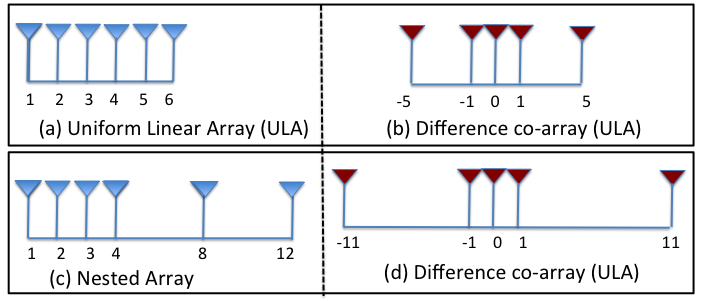
\includegraphics[width=0.5\columnwidth]{figs/FigNested.png}
\caption{\label{fig:Nested}  (a) A Uniform Linear Array with $6$ antennas and (b) its difference co-array with $11$ elements (c) A nested array with $6$ antennas and (d) its difference co-array with $23$ elements.}
%\vspace{-15mm}
%\subfigure{\includegraphics[width=2.5in]{GNS_Phase.eps}}
%\caption{Birds}
\end{figure}
We first motivate our sensor selection scheme by reviewing Co-PI Pal's prior work on sparse antenna array design, where the goal was to design {\em non-uniform} array geometries such that it is possible to localize more sources than the number of sensors \cite{PiyaNested,PiyaNested2D,PiyaCoprime,PalPushing}. 
This is provably not possible with uniform geometries, such as a uniform linear array (ULA). Consider the problem of estimating the directions of arrival (DOA) of $K$ far-field sources emitting narrowband plane-waves, using a linear array of $M$ sensors, where the $m$th sensor is located at a distance of $d_m$ (normalized with respect to the wavelength of source signals) from the origin. 
The sensing geometry and physical laws governing far-field wave propagation propagation together result in the following functional form for the map $\phi(.)$: \[ \phi(\mathbf{d},\theta_i,t) =  e^{j\pi d_m \sin\theta_i}s_i(t)  \]
%\[ y_m(t) = \sum_{i=1}^K {e^{j\pi d_m \sin\theta_i}s_i(t) + w_m(t) \] 
where $\theta_i$ is the DOA of the $i$th source and $s_i(t)$ is the corresponding baseband signal (which incurs negligible delay across the sensor array). Assuming that the source signals are statistically uncorrelated, the correlation between $m$th and $n$th sensors can be shown to be of them form \[ \mathbf{R}_{m,n} = \sum_{i=1}^{K}e^{j\pi (d_m-d_n)\sin\theta_i} p_i + \sigma^2_w\delta[m-n] \]
where $p_i$ is the power of the $i$th source and $\sigma^2_w$ is the noise power. 
It can be noted that the correlation {\bf only depends on the difference $d_m-d_n$ between sensor locations, and not on the actual locations $d_m$}. %As a special example, for a one dimensional antenna array receiving narrowband sources from spatial directions $r_k=\theta_k, 1\leq k\leq D$, we have $\phi(v_m,r_k)=e^{j\pi v_m\sin\theta_k}$. 
%Let $\mf{d}_m$ denote the spatial location of the $m$th antenna. 
%hen the sources of radiation are statistically uncorrelated, i.e. $E(s_k[l]s_j[l])=0, k\neq j$, the correlation between $y_m[l]$ and $y_n[l]$ can be shown to be a {\em function of the difference $\mf{v}_m-\mf{v}_n$}. 
Given the set $\mathcal{S} = \{d_1,d_2,\cdots, d_M\} $ of sensor locations,  we can associate a {\em difference set} $\mathbb{D}_{\mathcal{S}}$ as follows \[ \mathbb{D}_{\mathcal{S}}=\{d_m-d_n, d_m, d_n\in \mathcal{S} \} \] 
%If $\mathbf{a}(\theta)\in \mathbb{C}^{M\times 1}$ denotes the physical array steering vector, then the co-array steering vector is given by  \be \mathbf{a}_{ca}(\theta)=\mathbf{a}^{*}(\theta)\otimes\mathbf{a}(\theta)  \ee 
A traditional Uniform Linear Array (ULA) with $M$ antennas has only $2M-1$ elements in its difference set, as shown in Fig. \ref{fig:Nested} (a) and (b). In \cite{PiyaNested}, we proposed a new non-uniform array, namely the nested array, whose virtual array contains $O(M^2)$ elements. 
The nested array and its virtual array are depicted in Fig. \ref{fig:Nested} (c) and (d). In other words, given the same size of the virtual array, the nested array uses $O(\sqrt{M})$ antennas which results in {\em significant reduction in number of sensors} over Uniform Linear Arrays. This has paved the way for the possibility of localizing {\em more sources than sensors} purely by exploiting the geometry of sensing, and generated significant research interest in recent times both in terms of innovations in new sensing geometries \cite{GCA,han2014nested,hanTensor} as well new results in performance analysis in this regime \cite{koochakzadeh2016cramer,koochakzadeh2017performance,wang2017coarrays,tan2014direction}. \\


\noindent {\bf (b) \underline{Main Idea: Difference-set based Correlation Sketching and Sensor Subset Selection:}}
The idea of difference set inspired sampler design can be actually generalized beyond  antenna arrays, to acquire {\em compressive sketches} of the correlation between signals acquired between pairs of sensors. In general, given $N$ sensors, it is natural to think that one needs to compute the correlation between all $N\choose 2$ time series (from all possible sensor-pairs) to construct the overall $N\times N$ correlation matrix $\mathbf{R}$
%\footnote
(herein, $\mathbf{R}$ represents the ideal correlation matrix, whereas $\mathbf{\hat{R}}$ represents an estimate  computed with finite data).
However, using the idea of difference-set sampling, one can only compute  cross-correlation values between a much smaller subset of size $\sim\sqrt{N}$ of {\em suitably selected sensor-pairs} and recreate the entire $N\times N$ correlation matrix $\mathbf{R}$. In distributed sensing, this  means that only these sensors need to communicate and exchange information.

\noindent{\bf Approach: Exploiting Distance-based Redundancies Using Generalized Nested Samplers:} The main idea behind achieving such reduction is to exploit the redundancies present in the correlation values that naturally result from the physical spatial signal model. A widely used example of such a redundancy is that the correlation $\mathbf{R}_{m,n} = E\Big(y_m(t)y^*_n(t)\Big)$ between $m$th and $n$th sensors is of the following form %\begin{equation} 
\begin{equation} \mathbf{R}_{m,n} \approx f(\mathbf{d}_m - \mathbf{d_n}) \label{eqn:CorrRed} \end{equation}
%\end{equation}
Thus, the correlation is spatially only a function of the {\em inter-sensor displacement $\mathbf{d}_m - \mathbf{d_n}$}, and this is a direct consequence of the functional form of $\phi(.)$. This is also referred to as spatial stationarity and it is (exactly or approximately) true for many applications as narrowband and wideband radar \footnote{In the latter case, this holds at individual frequency bands after splitting the wideband signal into narrow frequency bins using a filter bank}, super-resolution optical imaging, mmWave wireless channels %\cite{} 
and so forth. Hence, depending on the inter-sensor distances, many of these $N\choose 2$ correlation values are actually repeated/redundant. Based on this observation, we propose using a new sketching technique developed by co-PI Pal, called {\bf Generalized Nested Sampling (GNS) to reduce the amount of inter-sensor communication} \cite{HP_letter,HP_GNS}. Suppose the sensors are located on a uniform grid. In one dimension, (\ref{eqn:CorrRed}) implies that the ideal correlation matrix $\mathbf{R}$ has Toeplitz structure and GNS provides an optimal way to select sensors to sketch such a matrix. The main idea is as follows. Select a subset $\mathcal{S}$ of sensors such that its difference set $\mathbb{D}_{\mathcal{S}}$ contains {\em all possible sensor locations of interest}. In other words, if we want $\mathbb{D}_{\mathcal{S}}$ to contain all possible locations of $N$ sensors, how should the set $\mathcal{S}$ be chosen so that it has minimal cardinality? GNS provides a simple yet effective way to select $\mathcal{S}$, which can be equivalently defined in terms of a {\em subset selection} matrix $\mathbf{A}_{\text{GNS}}$ whose structure dictates which $M$ sensors (out of $N$) are selected. % \cite{}.

%\noindent{\bf How GNS works} Given any integer $L\ge 6$, GNS is defined in terms of two integer valued parameters $\Theta(N)$ and $\Gamma(N)$ given by
%\begin{equation} \Theta(N) = \lfloor \sqrt{N + \frac{1}{4}} - \frac{1}{2} \rfloor \quad 
%\Gamma(N)=1+L-{\Theta}^2(N) 
%\end{equation}
%%The sampling matrix $\mathbf{A}$ called "Generalized Nested Sampling Matrix" in \cite{HP_GSip} is defined by
%Given $\Theta(N)$ and $\Gamma(N)$, a GNS can be defined as the following measurement/sensor-selection matrix
%\begin{definition} For any integer $N \ge 6$, a Generalized Nested Sampling matrix $\mathbf{A}_{\text{GNS}} \in \mathbb{R}^{M \times N}$, with $M = \Gamma(N) + \Theta(N) - 1$ is given by 
%
%\begin{equation}
% [\mathbf{A}_{\text{GNS}}]_{i,j}= \begin{cases}  1 & \textrm{if} \; j = i,\; 1 \le i \le \Gamma(N) \\
%1 & \textrm{if} \; j=(i-\Gamma(N))\Theta(N)+i, \quad \Gamma(N) < i \le M  \\
%0 &  \text{else}
%\end{cases}
%\label{def_A}
%\end{equation}
%\end{definition}
%Note that $\mathbf{A}_{\text{GNS}}$ is  a {\em row-selection} matrix that selects $M$ out of $N$ elements of a vector. 
In particular, the indices of these $M$ rows crucially tell us {\em which sensors to select} so that we  obtain a lossless sketch of $\mathbf{R}$ via  the cross-correlation between these $M$ sensors. Such selection is governed by the need to exploit distance-based redundancies as captured in (\ref{eqn:CorrRed}). As discussed earlier, when the sensors are located on a one uniform dimensional grid, (\ref{eqn:CorrRed}) essentially implies that the {\bf full correlation matrix $\mathbf{R}$ is a Toeplitz matrix}. %GNS dictates how to select a subset of $M$ sensors which maximally exploit the redundancies in a Toeplitz $\mathbf{R}$. 
%the number of rows of $\mathbf{A}_{\text{GNS}}$ scales . The specific case of $L=M^{2}/4+M/2-1$ was introduced as ``Nested Array" in \cite{PiyaNested}. As discussed in \cite{HP_GSip}, the fundamental idea behind GNS or other sparse ruler type sampler is to exploit the difference set of the sampling indices. In particular, each row of $\mathbf{A}_{s}$ contains a single $1$ and let $c(i)$ denote the index of the column containing it. Then, the $(i,j)$th entry of $\mathbf{R_Y}$ corresponds to $t_{c(i)-c(j)}$. The length of smallest range over which $(i,j)$ should be chosen so that $\{c(i)-c(j)\}$ spans all integers from $0$ to $L-1$ is $O(\sqrt{L})$ and the GNS shows a constructive way to select $c(i)$ over this range.
%\end{remark}
%%The following result from \cite{HP_GSip} shows how to compress a $N\times N$ Toeplitz matrix without assuming it to be low rank.
%\begin{lem}
%A real symmetric Toeplitz matrix $\mathbf{T}\in \mathbb{R}^{N \times N}$ can be exactly recovered from its compressed measurement $\mathbf{R_Y}=\mathbf{A}_{GNS}^{N} \mathbf{T}(\mathbf{A}_{GNS}^{N})^{T}$ where $\mathbf{A}_{GNS}^{N}\in \mathbb{R}^{M \times N}$ is a Generalized Nested Sampling Matrix given by (\ref{def_A}).
%\label{lem:general}
%\end{lem}
%\end{definition}
In particular, GNS dictates how to select a subset $\mathcal{S}_{\text{GNS}}$ of $M =  = \Theta(\sqrt{N})$ sensors out of $N$ available sensors so that the Toeplitz $\mathbf{R}$ can be {\em exactly reconstructed} from the pair-wise correlation between sensors in $\mathcal{S}_{\text{GNS}}$. Let $\mathbf{R}_{\mathcal{S}_{\text{GNS}}} \in \mathbb{C}^{M\times M}$ be the correlation matrix computed by aggregating the signals from these sensors. Then, we have 
\begin{equation}
\mathbf{R}_{\mathcal{S}_{\text{GNS}}} = \mathbf{A}_{\text{GNS}} \mathbf{R} \mathbf{A}^T_{\text{GNS}} 
\end{equation}
The structure of $\mathbf{A}_{\text{GNS}}$ ensures that $\mathbf{R}_{\mathcal{S}_{\text{GNS}}}$ is a {\em lossless} sketch of  $\mathbf{R}$. In turn, this tells us that ideally, it is sufficient for the $M$ sensors from $\mathcal{S}_{\text{GNS}}$ to communicate and exchange their measurements in order to  preserve the correlation information from all $N\choose 2$ sensor pairs. Since $M = \Theta(\sqrt{N})$, we can significantly reduce the cost of communication in a distributed sensor network by such correlation-aware sensor selection. Given the basic idea of GNS, we will focus on the following tasks to extend the capabilities of GNS to perform subset selection in two dimensions.
%\begin{enumerate}

\noindent{\bf (c) \underline{Proposed Research: Two Dimensional GNS and Hierarchical Sensor Selection:}} 
Most sensor networks of interest will be distributed over a two-dimensional area. Hence, it is important to extend the basic version of GNS (which was developed for sensors on a line) to two dimensions. In such cases, the geometry of sensor configurations have very interesting implications on the redundancy relation (\ref{eqn:CorrRed}) and the structure of $\mathbf{R}$. As an example, if we assume the sensors to be located on a uniform rectangular grid in two dimensions of size $N_x\times N_y$, then (\ref{eqn:CorrRed}) implies that $\mathbf{R}\in \mathbb{C}^{N_xN_y \times N_xN_y}$ is a {\em two-level} (or block) Toeplitz matrix. 
%of the form 
%\begin{equation}
%\mathbf{R} = \left[\begin{array}{cccc} \mathbf{T}_0 & \mathbf{T}_1 & \cdots & \mathbf{T}_{(N_y-1}) \\
%\mathbf{T}_{-1} & \mathbf{T}_0 & \cdots & \mathbf{T}_{(N_y-2)}\\
%\vdots & \vdots & \vdots & \vdots \\
%\mathbf{T}_{-(N_y-1)} & \mathbf{T}_{-(N_y-2)} & \cdots & \mathbf{T}_0 \end{array}\right]
%\label{eqn:2LevelToep} \end{equation}
%where $\mathbf{T}_i\in \mathbb{C}^{N_x\times N_x}$ is a Toeplitz matrix for each $i\in [0,N_y-1]$. 

\noindent We will develop two-dimensional versions of Generalized Nested Sampling (2D-GNS) to guide our sensor selection strategy so that we can produce a lossless sketch of $\mathbf{R}$ with far fewer sensors by exploiting its unique algebraic structure captured.% in (\ref{eqn:2LevelToep}). 
Notice that the extension is quite non-trivial given that $\mathbf{R}$ has Toeplitz structure in individual blocks, as well as the blocks are repeated along each (sub)-diagonal. The optimal sketching matrix should exploit the redundancies in both levels to produce a sketch of size $O(\sqrt{N_xN_y})$. 

\noindent {\bf Details of Two-dimensional GNS geometry on Lattices:} We will draw inspirations from our previous works in designing two-dimensional nested arrays \cite{PiyaNested2D} to develop the corresponding sketching 2D GNS operator $\mathbf{A}_{\text{2D-GNS}} \in \mathbb{R}^{M \times {N_xN_y}}$, where $M = O(\sqrt{N_xN_y})$. In particular, we propose to select $M=N_d+N_s$ sensors from a total of $N_xN_y$ sensors as follows. We choose a nonsingular {\em integer} matrix $\mathbf{P}\in \mathbb{Z}^{2\times 2}$ such that $\text{det}(\mathbf{P})=N_d$. The $N_s$ sensors belong to the following subset  of the uniform rectangular grid \[ \mathcal{S}_{s} = \{\mathbf{P}[n_1,n_2]^{T}, 0\leq n_1\leq N_1-1, 0\leq n_2\leq N_2-1 \} ,\quad N_1N_2 = N_s \]
and the $N_d$ sensors are located at \[ \mathcal{S}_d = \{ \mathbf{v} \in \text{FPD}(\mathbf{P}), \mathbf{v} \text{ is integer valued} \} \] 
%
Here $\text{FPD}(\mathbf{P})$ (aka Fundamental Parallelopiped of $\mathbf{P}$)  is the set of all vectors of the form $\{\mathbf{Px}, \mathbf{x}\in[0,1)^2 \}$. It can be verified that indeed the cardinality of $\mathcal{S}_d = \text{det}(\mathbf{P}) = N_d$. We further require $N_sN_d = N_xN_y$. Hence GNS selects a subset of sensors $\mathcal{S}_{\text{2D GNS}} = \mathcal{S}_s\cup \mathcal{S}_d$ which consists of a union of two subsets of the original lattice: (i) $\mathcal{S}_d$ consisting of $N_d$ densely spaced sensors on a rectangular grid, and (ii) $\mathcal{S}_s$ consisting of $N_s = N_1N_2$ sensors on a larger (sparser) lattice generated by the integer matrix $\mathbf{P}$ (which is also a sub-lattice of the desired uniform rectangular grid). The vector difference set $\{\mathbf{d}_m-\mathbf{d}_n, \mathbf{d}_m,\mathbf{d}_n\in \mathcal{S}_{\text{2D GNS}}\}$ consists of all $N_xN_y$ consecutive integer points on the 2D rectangular lattice. Using this property of 2D Nested arrays, we will develop the corresponding sketching matrix $\mathbf{A}_{2D GNS}$ and develop an effective way to sketch the two-level Toeplitz structured $\mathbf{R}$ using only $M = O(\sqrt{N_xN_y})$ communicating sensors. 

An interesting aspect of our design is that it will use a combination of closely spaced sensors (given by $\mathcal{S}_d$) and far-apart sensors (given by $\mathcal{S}_s$). This will naturally have two advantages. 
Firstly,  it is well known that for passive sensing, sensor pairs that are further away automatically provide larger time delays of arrival between signals from two different sources, thereby resulting in higher accuracy of detection (and better spatial resolution). However, if the source is farther away from each sensing unit, the longer path loss can result in degraded signal-to-noise ratio (SNR). The proposed 2D GNS sampler provides a balance between these two aspects by using a combination of both close and far sensors. Such an architecture will lead to development of efficient algorithms that will utilize the higher spatial resolution offered by the array of distant sensors and counterbalance the effect of low SNR and ambiguity by utilizing the structure of the smaller and denser array. 

A second interesting aspect of 2D GNS is that it lends itself to a hierarchical selection of communicating sensors, depending on how many targets to detect, and how large the field of view is. For example, we can divide a wide field of view into smaller segments. Depending on which segment captures the target of interest 
%\footnote{There can be several criterion for determining this. A simple option would be to divide the sectors based on received signal strength},
we can zoom into that part and determine the subset of communicating sensors using the 2D GNS-based subset selection rule. We can implement such subset selection by dynamically turning sensors on and off. Alternatively, in a multi-target environment where the targets are sufficiently far apart, we can dedicate different segments to localize different targets and dynamically select the communicating sensors from each segment. Finally, it is to be noted that the orientation of the communicating sensors on the lattice is determined by the integer matrix $\mathbf{P}$ and such orientation can affect target localization performance (especially the source angles). When we have partial knowledge of target location, it will also be of interest to design $\mathbf{P}$ to orient the subset so as to maximize the target detection probability. For multi-target scenario, we can design different $\mathbf{P}$ matrices (if needed) for each of the aforementioned segments.

\yoav{plopped this here, because I wanted it inside the section regarding selection of a subset of the ssensors}
\piya{I think we should move them to the beginning of proposed task so that the reviewers know that proposed task actually answers these questions}


% We will develop the corresponding structure of the 2D GNS sketching matrix and understand 

%item {\bf Finite Sample Performance:} 
%\item {\bf Wideband Signal and Spatio-temporal GNS:}

%\end{enumerate}
%\piya{To Add (i) Finite sample performance guarantees (ii) two and three-dimensional extension: Subsets of regions where targets are tracked, split into regions where GNS is employed to reconstruct the individual scenes (Cellular system like), (iii) Wideband Signals (iv) Time-varying model.}


%Will focus on what subsets of sensors in a distributed setting should communicate to be able to reconstruct the source scene. Can think of a subset of spatially close sensors to fully communicate with each other (assuming cost of communication proportional to proximity/distance), and then transmit the sketch / coarse parameter estimates (or their binarized measurement) to the sensors further away. Can lead to interesting hierarchical configurations for distributed sensors, dictated by $\phi(.)$. {\color{red} [To Add more Details..]}.
%\yoav{I think this is a very interesting question. Especially when the best subset depends on the location of the source.}\rayan{agree!}
%\item {\em Beyond Point Target Localization: Using Priors and Sparsity} In many applications such as camera networks, the quantities of interest are not the low-level measurements acquired at the CCD sensors, but the processed images $I_t$. In such cases, we need to obtain a compressive sketch of the image $A (I_t)$ via the sketching operator $A (.)$ using low dimensional representation (over unions of subspaces or manifolds). In addition to conventional sparsity and low-rank priors, one can also utilize (partial) knowledge of the prior distribution of the images $I_t\sim~\mathcal{D}$. Utilizing these priors can lead to more effective compression for a given level of sparsity. {\color{red} [To be written..]}  
%\end{enumerate}
\piya{These tasks can be further integrated with the binary embedding based sketching ideas proposed by Rayan and Alex.}
\rayan{Agree!}
%\end{itemize}
